	\subsection{Taxonomy of Virtualization Tools by \textit{Abdulhamid}}
	
	\begin{figure}[H]
		\centering
		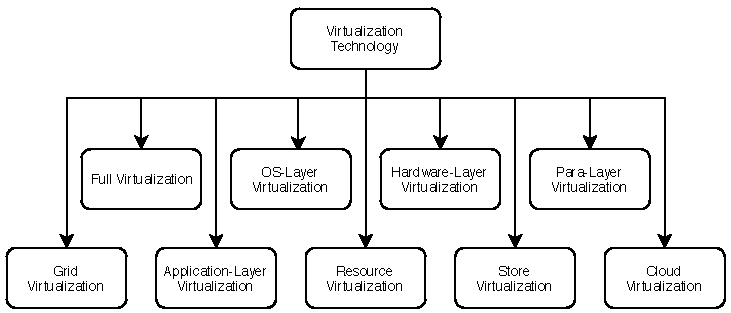
\includegraphics[width=8.5cm]{images/Abdulhamid2014.pdf}
		\vspace{-0.2cm}
		\caption{Taxonomy of virtualization tools by \textit{Shafi'i Muhammad Abdulhamid, Muhanmmad Shafie Abd Latiff and Mohammed Bakri Bashir} in 2014 \cite{Abdulhamid2014}.}
		\label{fig:TaxonomyByAbdulhamid}
	\end{figure}
	
	In the work of \textit{Abdulhamid} \cite{Abdulhamid2014} a taxonomy is presented whose purpose is to classify the hypervisors under the virtualization technology from the point of view of resource provisioning in cloud computing. This initiative is supported by the boom in cloud computing, particularly infrastructure as a service (IaaS). This purpose is based on the work of Sahoo, et al \cite{Sahoo2010}, which had the following seven categories: \textit{a) Full Virtualization}, \textit{b) OS-Layer Virtualization}, \textit{c) Hardware-Layer Virtualization}, \textit{d) Para virtualization}, \textit{e) Application virtualization}, \textit{f) Resource virtualization}, \textit{g) Storage virtualization}. In addition, \textit{Abdulhamid's} work adds the followings two categories: \textit{h) Grid virtualization} and \textit{i) Cloud virtualization}. See Figure \ref{fig:TaxonomyByAbdulhamid}. Some of the categories proposed here have already been described, so below is brief description of only some of the remaining. 
	
	\textbf{Resource virtualization}: this type refers to the virtualization of a computer system such as storage volumes, name spaces and networks \cite{Abdulhamid2014}.	Some of the methods used to implement this type of virtualization are the following: a) Combining several components in a larger pool of resources, b) Clusters of high-performance computers and c) separating a resource many smaller resources.
	
	\textbf{Grid virtualization}: This type focuses on virtualization of a grid resources either for the Virtual Organization (VO) or for a Virtual Organization Cluster (VOC). The general aim then is that hardware administrators can retain control of VMMs, as coarse grain resource sharing and monitoring can be executed by VM.
	
	\textbf{Cloud virtualization}: In recent times, the cloud computing paradigm has made it possible to offer on-demand provisioning of virtual resources through the web and applying the concept of pay-per-use. As a result of the above, virtualization now forms the basis of Cloud Computing, as it provides the ability to combine computing resources from clusters or networks and the provisioning of VM resources to customers on demand \cite{Abdulhamid2014, Aceto2013}.
	
	
	Although the work presented by \textit{Abdulhamid et al}. \cite{Abdulhamid2014} shows a graph suggesting two levels (See Figure \ref{fig:TaxonomyByAbdulhamid}), from a hierarchical perspective only one level can be observed comprising its nine categories. On the other hand, the description that presents the categories to the very superficial and also lacks concrete examples of technologies that belong to each category described. 
	
	
